%
% Complete documentation on the extended LaTeX markup used for Insight
% documentation is available in ``Documenting Insight'', which is part
% of the standard documentation for Insight.  It may be found online
% at:
%
%     http://www.itk.org/

\documentclass{InsightHowto}
\usepackage[dvips]{graphicx}
\usepackage{amsmath}

\title{How-To Create a Symmetric Ellipsoid Image Using itkEllipsoidInteriorExteriorSpatialFunction}

\release{0.01}

% At minimum, give your name and an email address.  You can include a
% snail-mail address if you like.
\author{Robert J. Tamburo}

\authoraddress{
University of Pittsburgh\\
749 Benedum Hall\\
Pittsburgh, PA 15261\\
rjtst21@pitt.edu}

\begin{document}

\maketitle

% This makes the Abstract go on a separate page in the HTML version;
% if a copyright notice is used, it should go immediately after this.
%
\input{Copyright.tex}

\ifhtml
\chapter*{Front Matter\label{front}}
\fi

% The abstract should be a paragraph or two long, and describe the
% scope of the document.
\begin{abstract}
\noindent This example demonstrates how to create a geometrical shape within an
\emph{itkImage} using Spatial Functions. Specifically, this example will use
\emph{itkSymmetricEllipsoidInteriorExteriorSpatialFunction} to create an itkImage consisting
of a symmetric ellipsoid along an orientation vector.  An n-dimensional symmetric ellipsoid
is one, which has $m$ axes of equal length and $(n-m)$ unique axes lengths.  Specifically,
itkSymmetricEllipsoidInteriorExteriorSpatialFunction creates a symmetric ellipsoid for the
case where $(n-m)=1$ and the ellipsoid's major axis is oriented along a single orientation
vector. itkSymmetricEllipsoidInteriorExteriorSpatialFunction creates a symmetric ellipsoid
for the can be found in the \module{functions} module.
\end{abstract}

\tableofcontents

\section{Example Description}

First, an \emph{itkImage} $\big($dimension of $3$, size of $50x50x50$, spacing of $(1,1,1)$,
and origin $(0,0,0)$ $\big)$ is created and completely filled with pixels of intensity value
$128$. Then, \emph{itkFloodFilledSpatialFunctionConditionalIterator} is used to iterate
through the image and set pixels to 256 if
\emph{itkSymmetricEllipsoidInteriorExteriorSpatialFunction} returns 1, meaning that it is
within the interior of the ellipsoid. The ellipsoid is defined by its axes lengths (from
edge-to-edge of the ellipsoid) as well as the orientations of its unique axes. This example
is restricted to 3D to allow for the visualization of the resulting image, which is done via
a \emph{VTK} image. The volume of the ellipsoid is measured by counting the number of
interior pixels of the ellipsoid. This measure can be used to verify the resulting ellipsoid
by comparing it against the calculated volume (percent difference) of the ellipsoid given
by:
\begin{equation}\label{1}
  V=\frac{4}{3} \pi \Big(\frac{a}{2}\Big) \Big(\frac{b}{2}\Big) \Big(\frac{c}{2}\Big),
\end{equation}
where a, b, and c are the lengths of the ellipsoid axes.

The ellipsoid is also validated by checking that the center of the ellipsoid has been
labeled as an interior pixel (a function value of 1) by evaluating the spatial function at
the origin of the ellipsoid.

Note: Orientation vector must be normalized!

\section{What is Needed to Run This Example?}

Build and run itkSymmetricEllipsoidInteriorExteriorSpatialFunctionExample.cxx from the
workspace generated from CMake. The resulting VTK image file is stored as:

\begin{center}
"Insight/Applications/SymmetricEllipsoidInteriorExteriorSpatialFunction/symmetricEllipsoid.vtk"
\end{center}

Default settings should result in an image of an ellipsoid with its axis Default settings
should result in an image of an ellipsoid with its unique axis of length 45 oriented along
the (1,1,0) direction and symmetric axes of length 30. The origin of the ellipsoid is
sampled and evaluated by the spatial function and returns \emph{function value}, which is 1
since the origin of the ellipsoid is within the ellipsoid.

   \begin{center}
   Results of the example (with defaults):\\
   \begin{tabular}{|c|c|}  % start the table
                     % two columns "c" centered
   \hline            % top line of the table
   calculated ellipsoid volume & 21205.8 pixels \\
   \hline
   measured ellipsoid volume & 21197 pixels \\
   \hline
   volume error & 0.04123 \% \\
   \hline
   function value  &  1 \\
   \hline
   \end{tabular}
   \end{center}

\begin{figure}[!hbp]
       \centering
       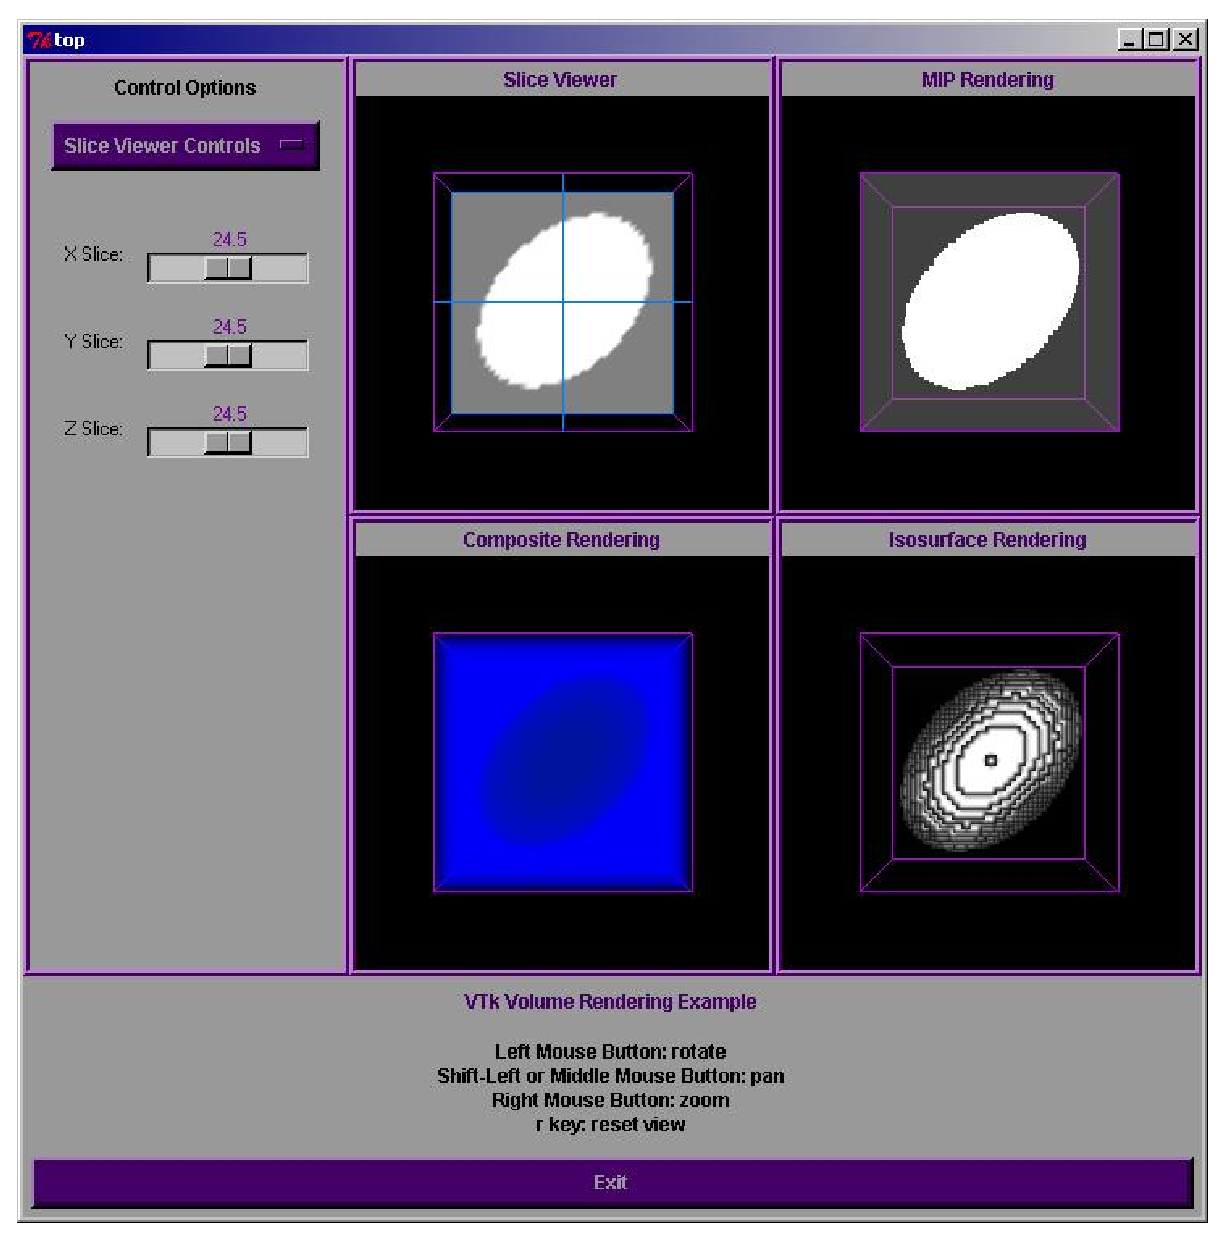
\includegraphics[width=.7\textwidth]{symmetricEllipsoid.eps}
       \caption{Resulting Image Containing an Ellipsoid From This Example \label{Fig. 1.} }
\end{figure}

*See Fig. 1 below or
"Insight/Applications/SymmetricEllipsoidInteriorExteriorSpatialFunction/symmetricEllipsoid.jpg"
for snapshot of resulting image.

\section{Insight Classes Used}

These are the Insight classes used for this example with a brief description. They appear in
order of first use:

\begin{itemize}
\item itkImage.h: generates a physical image.
\item itkImageRegionIterator.h: iterates through the pixels in the physical image and sets
them to $128$.
\item itkSymmetricEllipsoidInteriorExteriorSpatialFunction.h: evaluates pixels in the image and determines whether they are within the symmetric ellipsoid or
not.
\item itkFloodFilledSpatialFunctionConditionalIterator.h: iterates the image and sets them to $256$ if they are within the
ellipsoid.
\end{itemize}

\section{Possible Uses Of Ellipsoids}
The ellipsoid images created by SymmetricEllipsoidInteriorExteriorSpatialFunction are useful
for testing imaging algorithms, pixel sampling routines, establishing geometric domains of
influence, etc. Symmetric ellipsoids are useful where only one orientation vector is known
and minor axes of equal lengths are tolerable.

\section{Non-ITK Requirements}
A VTK image viewer is needed to visualize the output file symmetricEllipsoid.vtk.

\section{Copyright}
Copyright \copyright 2001 Insight Consortium All rights reserved.

Redistribution and use in source and binary forms, with or without modification, are
permitted provided that the following conditions are met:

 * Redistributions of source code must retain the above copyright notice,
   this list of conditions and the following disclaimer.

 * Redistributions in binary form must reproduce the above copyright notice,
   this list of conditions and the following disclaimer in the documentation
   and/or other materials provided with the distribution.

 * The name of the Insight Consortium, nor the names of any consortium members,
   nor of any contributors, may be used to endorse or promote products derived
   from this software without specific prior written permission.

  * Modified source versions must be plainly marked as such, and must not be
    misrepresented as being the original software.

THIS SOFTWARE IS PROVIDED BY THE COPYRIGHT HOLDER AND CONTRIBUTORS ``AS IS'' AND ANY EXPRESS
OR IMPLIED WARRANTIES, INCLUDING, BUT NOT LIMITED TO, THE IMPLIED WARRANTIES OF
MERCHANTABILITY AND FITNESS FOR A PARTICULAR PURPOSE ARE DISCLAIMED. IN NO EVENT SHALL THE
AUTHORS OR CONTRIBUTORS BE LIABLE FOR ANY DIRECT, INDIRECT, INCIDENTAL, SPECIAL, EXEMPLARY,
OR CONSEQUENTIAL DAMAGES (INCLUDING, BUT NOT LIMITED TO, PROCUREMENT OF SUBSTITUTE GOODS OR
SERVICES; LOSS OF USE, DATA, OR PROFITS; OR BUSINESS INTERRUPTION) HOWEVER CAUSED AND ON ANY
THEORY OF LIABILITY, WHETHER IN CONTRACT, STRICT LIABILITY, OR TORT (INCLUDING NEGLIGENCE OR
OTHERWISE) ARISING IN ANY WAY OUT OF THE USE OF THIS SOFTWARE, EVEN IF ADVISED OF THE
POSSIBILITY OF SUCH DAMAGE.

\end{document}
